\chapter{Introduction}

\section{Background: Dark Patterns in Mobile Interfaces}

Mobile applications have become one of the primary environments in which users search for information, purchase goods, order services, consume media, and manage social relationships. In these environments, interface design does not merely present information neutrally. It also structures attention, determines which options are visible, decides how much effort is required to reject an offer, and shapes the sequence of actions through which a user reaches a decision. When such interface structures are used to steer, coerce, or mislead users into decisions they may not have intended, they are commonly referred to as dark patterns or deceptive user interfaces \cite{gray2018darkpatterns,mathur2019darkpatterns}.

Dark patterns can appear in many forms. A shopping application may highlight a large, colorful button for accepting an add-on while hiding the decline option in small text. A subscription service may make registration simple but cancellation slow, confusing, or multi-step. A mobile game may repeatedly show pop-ups that interrupt normal interaction until the user accepts a promotion. A food-delivery or e-commerce platform may show countdown timers, scarcity messages, or limited-time claims that create pressure during the decision process. Other examples include hidden close buttons, preselected add-ons, forced login before viewing content, repeated notification prompts, or interface flows in which the easier path benefits the platform rather than the user. Although these examples differ in appearance, they share a common feature: the interface changes the user’s decision environment in a way that may reduce informed, voluntary, or frictionless choice.

Prior research has made important progress in defining and categorizing these practices. Early work in human-computer interaction framed dark patterns as a design ethics problem, emphasizing how interface choices can conflict with user autonomy and welfare \cite{gray2018darkpatterns}. Later empirical studies showed that dark patterns are not isolated anecdotes but measurable phenomena that can be systematically identified and categorized across large numbers of websites and applications \cite{mathur2019darkpatterns}. Other work further connects dark patterns to the manipulation of choice architecture, arguing that deceptive interfaces should be analyzed not only by their visual appearance but also by how they modify available options, information flow, and decision costs \cite{mathur2021whatmakesdark}. These studies provide the conceptual foundation for treating dark patterns as observable and measurable interface phenomena.

However, mobile applications introduce additional complexity. Compared with static web pages, mobile apps are often highly interactive, personalized, and session-dependent. A user’s interface trajectory may depend on search terms, browsing behavior, click history, location-sensitive services, payment-related actions, and recommendation feedback. Therefore, a dark pattern may not be equally visible to all users at all times. It may appear only after a user searches for a certain keyword, opens a decision page, enters a checkout flow, or repeatedly rejects a prompt. This motivates a shift from asking only whether dark patterns exist in an application to asking how users are exposed to them during actual interaction.

\section{From Dark Pattern Presence to User Exposure}

Much of the existing literature has focused on the presence, taxonomy, and detection of dark patterns. This line of work is essential because it makes deceptive design visible and measurable. Taxonomies help researchers name recurring mechanisms such as obstruction, sneaking, nagging, forced action, interface interference, urgency, scarcity, and social proof \cite{gray2018darkpatterns,mathur2019darkpatterns}. Large-scale measurement studies further demonstrate that such patterns can be counted, classified, and compared across digital services \cite{mathur2019darkpatterns}. Consent-interface studies also show that seemingly small differences in button placement, default settings, or rejection paths can significantly alter user choices \cite{nouwens2020gdpr}. Together, these studies establish that dark patterns are not merely subjective impressions; they can be operationalized as empirical objects.

Nevertheless, the presence-based perspective has limitations for mobile app auditing. If a researcher records that an application contains a countdown timer, a forced login gate, or a difficult cancellation flow, this does not fully answer which users encounter that mechanism, under what interaction conditions, and how often it appears along a realistic interaction path. A dark pattern that exists deep inside a checkout process may be irrelevant to a casual browsing user but highly relevant to a user who repeatedly opens payment pages. Similarly, repeated pop-ups may appear only after certain categories of interaction, while promotional pressure may depend on whether the user searches for discount-related or high-value products.

For this reason, this report treats dark patterns not only as interface-level objects but also as exposure events. Exposure refers to the observed encounter between a user profile, an interaction trajectory, and a dark-pattern mechanism. This view is especially important in mobile applications because the interface is not a single static artifact. It is a sequence of screens, prompts, recommendations, pop-ups, and decisions. The same app may expose different users to different combinations of friction, pressure, forced action, sneaking, or contextual deception depending on how they interact with it. Therefore, the key measurement problem becomes conditional: given a controlled user profile \(A\), what level and type of dark pattern exposure \(D\) is observed? In this report, this relationship is expressed as profile-conditioned exposure estimation, denoted as \(E(D \mid A)\).

This exposure-based framing does not require claiming that applications intentionally target specific users with dark patterns. Instead, it asks a more limited and empirically observable question: when controlled profiles interact with the same applications under reproducible procedures, do their observed dark-pattern exposure patterns differ? This distinction is important. The framework developed in this project measures profile-conditioned exposure, not developer intention or causal targeting. It is designed to provide evidence about differential interface experience while avoiding unsupported claims about why those differences occur.

\section{Personalization as a Missing Dimension}

The motivation for profile-aware dark pattern auditing comes from the broader role of personalization in digital platforms. Modern mobile applications routinely personalize recommendations, rankings, advertisements, promotional interfaces, and interaction flows. Search results may vary based on prior behavior, recommendation feeds may change after repeated clicks, and promotional prompts may be triggered by inferred interests or decision-stage actions. Prior work on personalization has shown that different users can receive different outputs from the same platform, even when the visible task appears similar \cite{hannak2013personalization}. Algorithm auditing research has also demonstrated that controlled user profiles can be used to study differential exposure in search engines, recommendation systems, and online platforms whose internal mechanisms are not directly accessible to researchers \cite{sandvig2014auditing,ribeiro2020auditing,haroon2023youtubeaudit}.

This project applies that auditing logic to deceptive interface exposure. If platforms personalize content and interaction flows, then users with different interest and behavior profiles may not experience the same sequence of screens. A high-payment shopping profile may frequently search for expensive products, browse high-value items, and enter payment-related pages. A low-payment browsing profile may spend more time scrolling, viewing general content, and avoiding checkout flows. A bargain-hunter profile may search for coupons, discounts, group-buying options, and flash-sale promotions. These profiles are not intended to represent demographic groups. Instead, they are controlled experimental abstractions that capture different interest distributions and behavior distributions.

The exclusion of demographic attributes is a deliberate design choice. Demographic variables such as age, gender, or identity attributes are difficult to control ethically and reproducibly in a course-scale audit. They may also introduce unnecessary privacy and fairness concerns. By contrast, interests and behaviors can be operationalized through observable interaction choices: what keywords a profile searches for, how frequently it browses, whether it opens decision interfaces, and how often it interacts with recommendation or payment-related pages. This allows the audit to focus on profile-conditioned exposure without making claims about protected demographic groups.

The central assumption is therefore modest but important: because mobile applications often adapt to user behavior and interest signals, different controlled profiles may follow different interface trajectories and may consequently encounter different dark-pattern mechanisms. A high-payment profile and a bargain-hunter profile may both be more likely to reach promotional or decision-oriented screens, while a low-payment browsing profile may remain more often in general browsing contexts. These differences may be associated with different levels of interface interference, pressure, forced action, or other DPS dimensions. The purpose of the framework is to measure whether such differences are observable and statistically supported, not to infer the internal logic of the applications.

\begin{figure}[htbp]
    \centering
    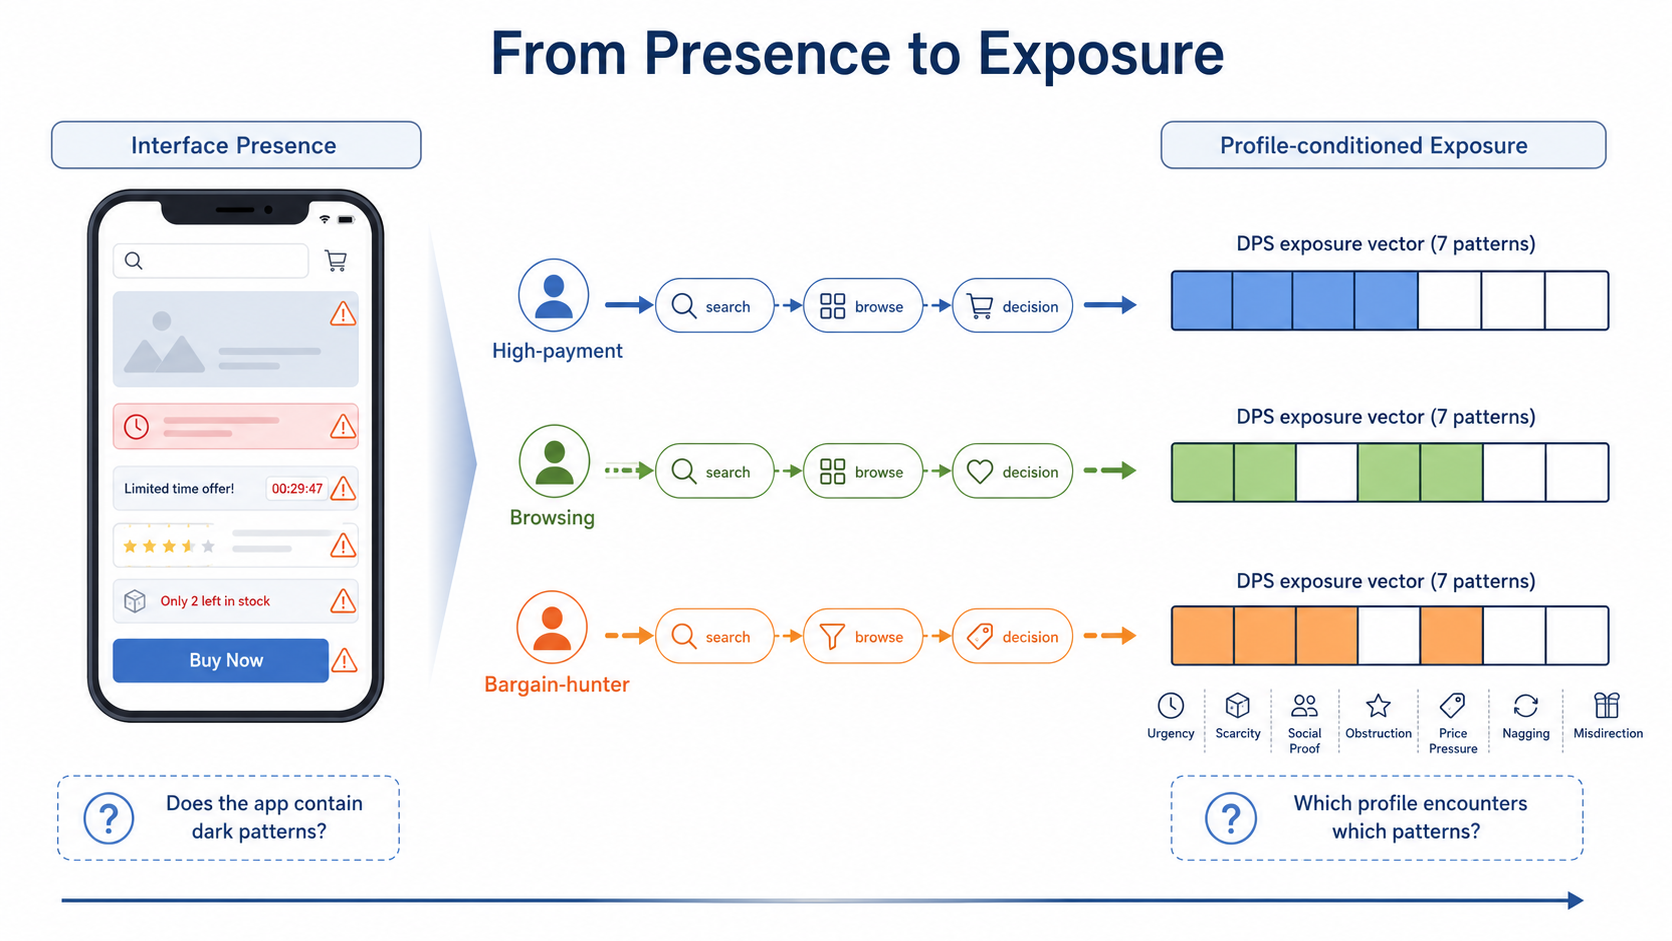
\includegraphics[width=0.95\linewidth]{figures/pictures/presence_to_exposure.png}
    \caption{From Dark Pattern Presence to Profile-Conditioned Exposure.}
    \label{fig:presence-to-exposure}
\end{figure}

\section{Research Questions}

Based on the above motivation, this report investigates personalized dark pattern exposure in mobile applications through a profile-aware auditing framework. The study is organized around four research questions.

\begin{enumerate}
\item \textbf{RQ1: Do different user profiles experience different dark pattern exposure during mobile app interactions?}
This question examines whether controlled profiles produce different observed exposure patterns when interacting with the same set of applications. The focus is not simply on whether an app contains dark patterns, but on whether exposure varies across profile-conditioned interaction trajectories.

\item \textbf{RQ2: Can dark pattern exposure be operationalized as a multidimensional annotation vector suitable for comparison?}  
This question concerns measurement design. Instead of assigning only a single binary label to each screenshot, the project annotates each interaction record using a seven-dimensional Dark Pattern Score vector, \(\mathrm{DPS} = [I, F, P, C, S, N, FA]\), where \(I\) denotes Interface Interference, \(F\) denotes Friction, \(P\) denotes Pressure, \(C\) denotes Contextual Deception, \(S\) denotes Sneaking, \(N\) denotes Nagging, and \(FA\) denotes Forced Action.

\item \textbf{RQ3: Do exposure estimates stabilize over repeated interactions?}  
Since dark pattern exposure may vary from step to step, a single screenshot may not provide a reliable basis for comparison. This question evaluates whether running mean exposure estimates gradually stabilize over repeated interactions, supporting the use of fixed-step exploration trajectories.

\item \textbf{RQ4: Can statistical validation show that observed exposure differences exceed random variation?}  
This question asks whether the measured differences across profiles are larger than what would be expected under random profile assignment. The analysis uses permutation tests, q-values, L1 distance, and Cramér’s V to assess statistical significance and practical association.

\end{enumerate}

\section{Contributions}

This report makes five main contributions. First, it proposes a profile-aware auditing framework for measuring dark pattern exposure in mobile applications. Rather than treating dark patterns only as static interface elements, the framework measures them as observed exposure outcomes along controlled interaction trajectories. This allows the analysis to compare \(E(D \mid A)\), the expected exposure vector conditioned on a user profile \(A\).

Second, the report introduces a controlled profile construction method based on interest and behavior distributions. Interests are represented as probability distributions over keywords, while behaviors are represented as probability distributions over interaction actions. This design makes the profiles reproducible and suitable for black-box auditing, while avoiding demographic attributes that are harder to control and may raise additional ethical concerns.

Third, the report operationalizes dark pattern exposure using a seven-dimensional DPS vector. The vector summarizes key mechanisms discussed in prior dark pattern taxonomies, including interface interference, friction, pressure, contextual deception, sneaking, nagging, and forced action \cite{gray2018darkpatterns,mathur2019darkpatterns,mathur2021whatmakesdark}. This multidimensional representation is more informative than a single presence label because it captures the type of manipulative mechanism encountered in each interaction record.

Fourth, the report presents an empirical audit design involving 16 apps, 3 profiles, and 30 interaction steps per profile-app pair, resulting in 1{,}440 interaction records. Since each record is annotated across seven DPS dimensions, the complete dataset contains 10{,}080 DPS labels. The implementation chapter describes the audit pipeline, while Chapter~\ref{sec:experimental-design} summarizes the experimental scale and annotation structure.

Fifth, the report provides evidence that dark pattern auditing should move beyond interface-level detection toward profile-aware differential exposure analysis. The findings suggest that different profiles show different DPS exposure patterns, that exposure estimates gradually stabilize after repeated interactions, and that statistical validation supports the presence of profile-dependent exposure differences. In particular, the high-payment and bargain-hunter profiles are associated with stronger interface interference and pressure-related exposure, while some app categories, such as food-delivery apps, show consistently high forced-action exposure. These findings do not prove intentional targeting by applications. Rather, they indicate that observed dark pattern exposure may depend on the profile-conditioned interaction trajectory. This perspective expands dark pattern research from the question of whether deceptive interfaces exist to the question of who encounters which mechanisms, under what conditions, and with what measurable differences.
